\def\annoBubbleRadius{1cm}

\subtikzpicturedef{subCADExhaustCMODE} {
    origin%
} {
    \draw (#1-start) coordinate (#1-origin);

    \draw
    (#1-origin)
    node (#1-imgTop) [
        inner sep = 0pt,
        anchor = center,
    ] {
        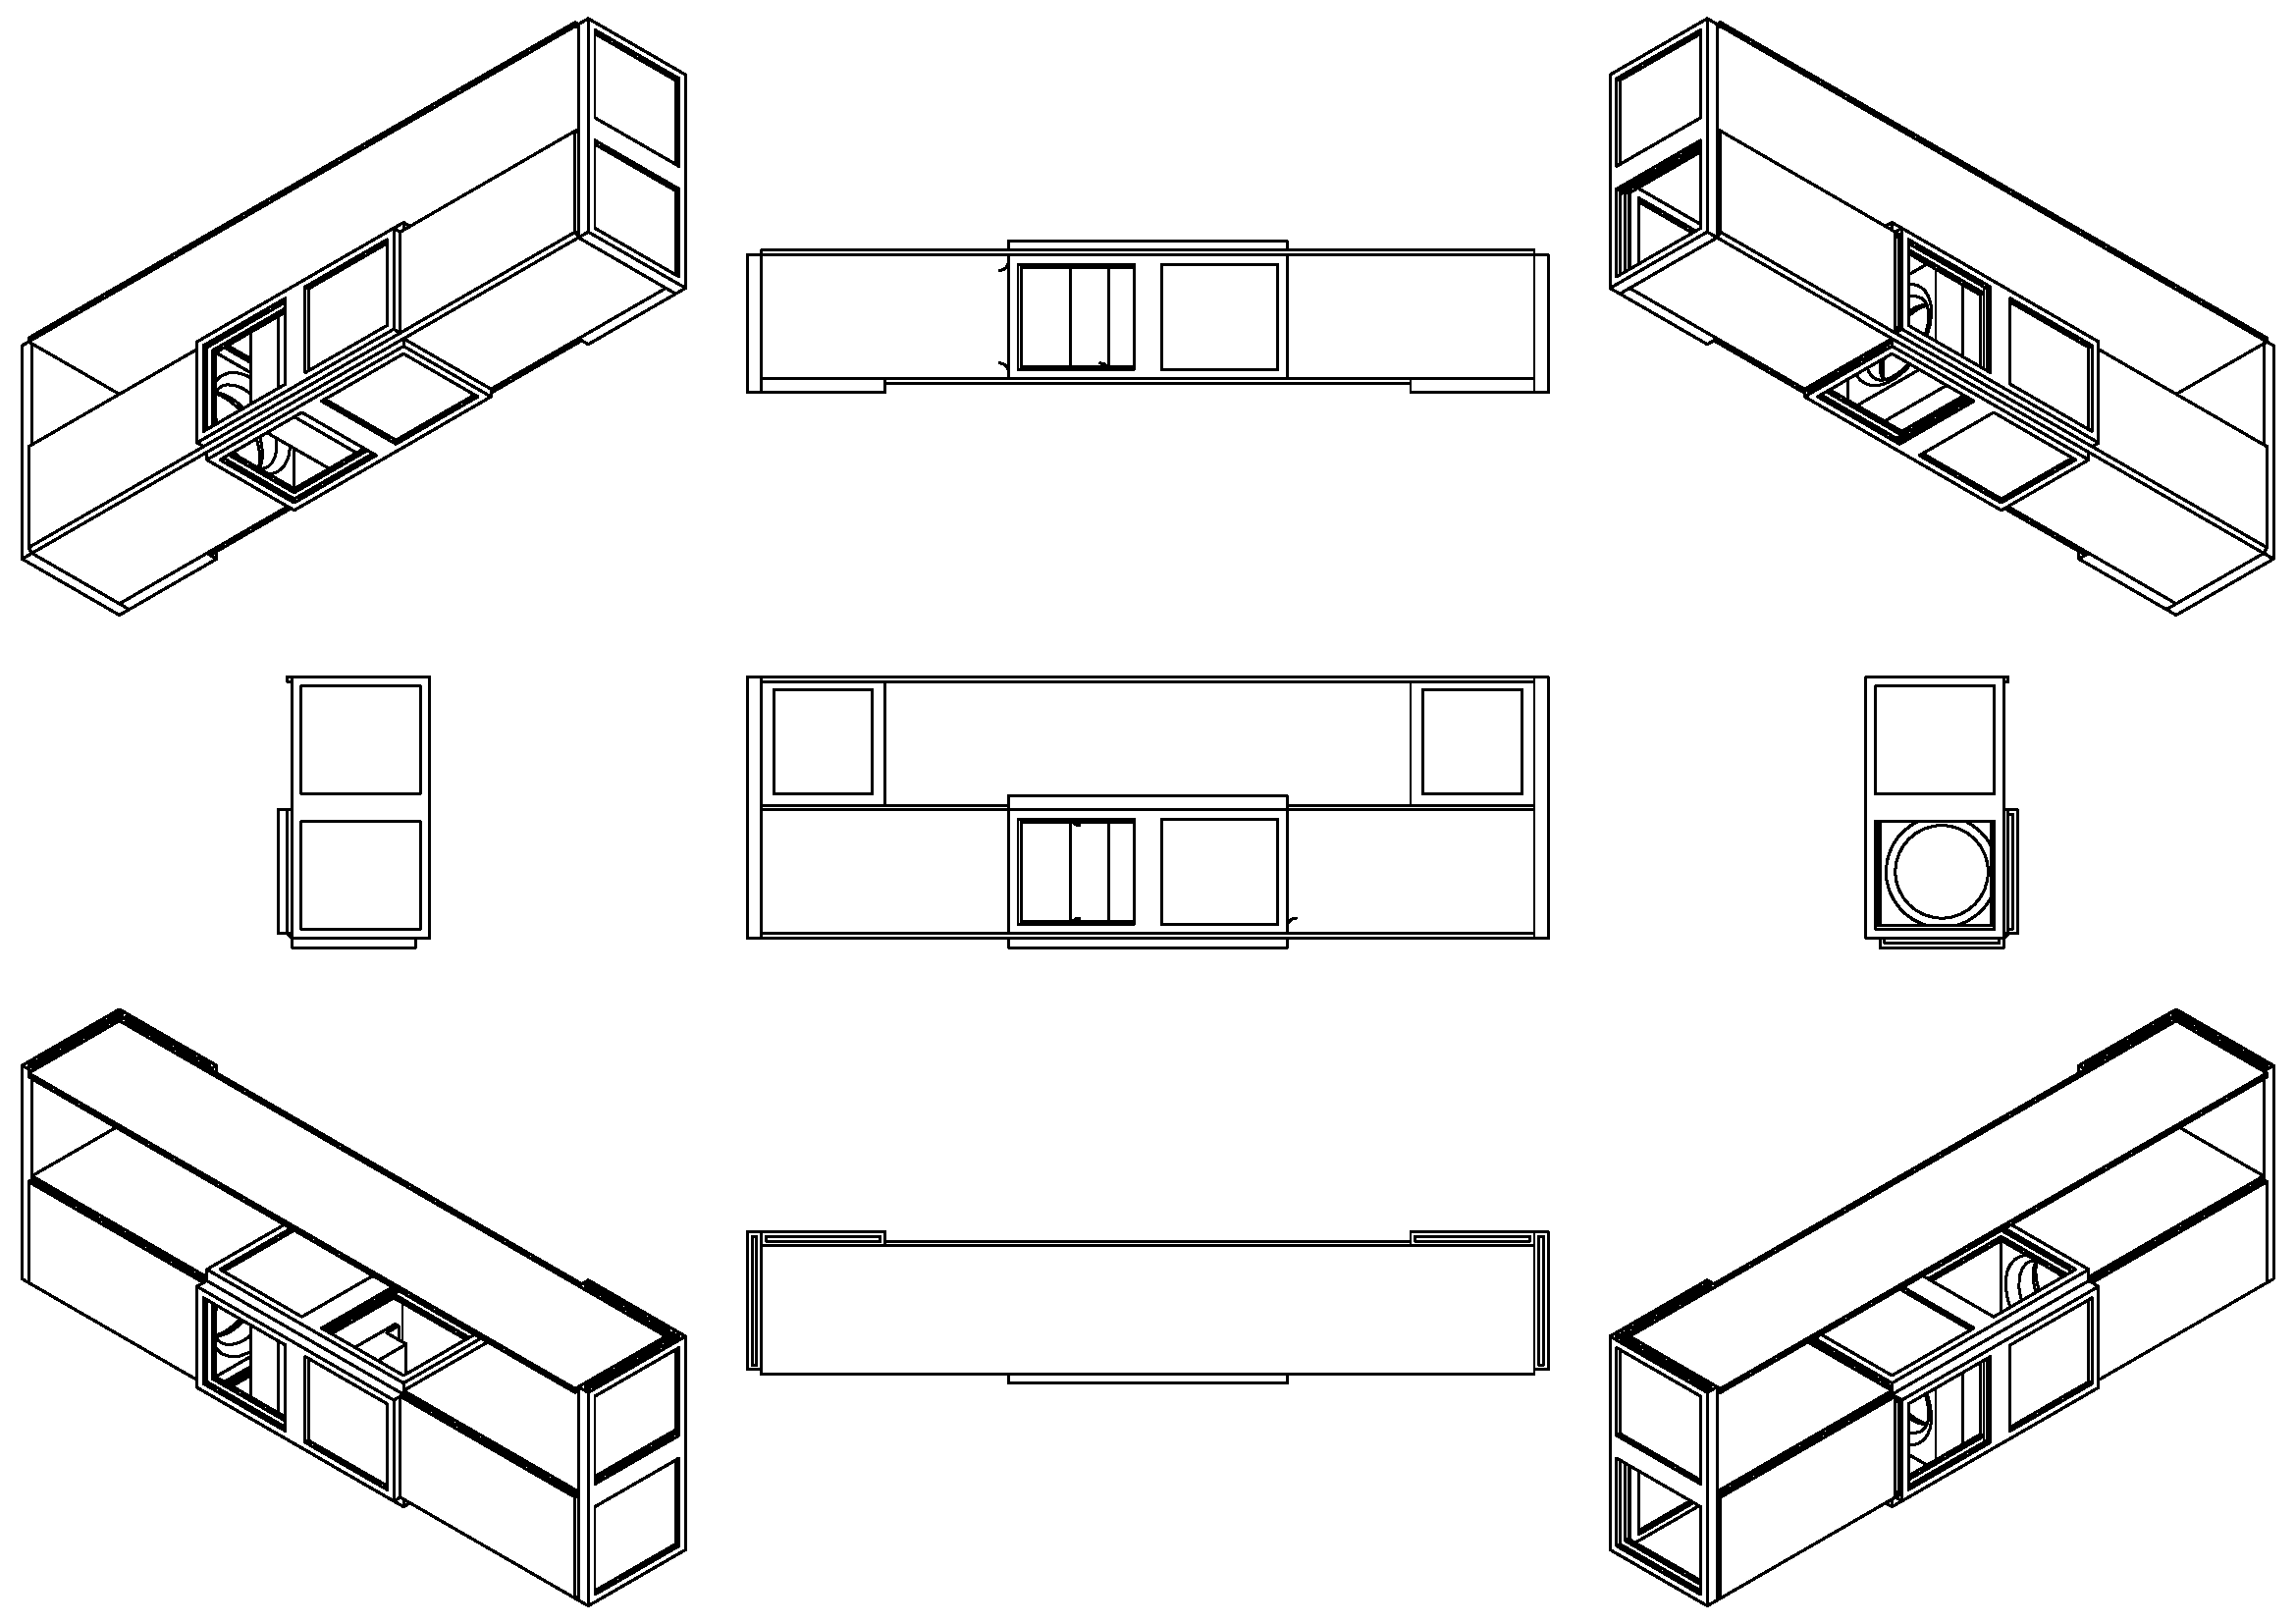
\includegraphics [
        ] {\subfix{pics/cmode_top.pdf}}
    }

    (#1-imgTop.south) ++(0, -1cm)
    node (#1-imgBot) [
        inner sep = 0pt,
        anchor = north,
    ] {
        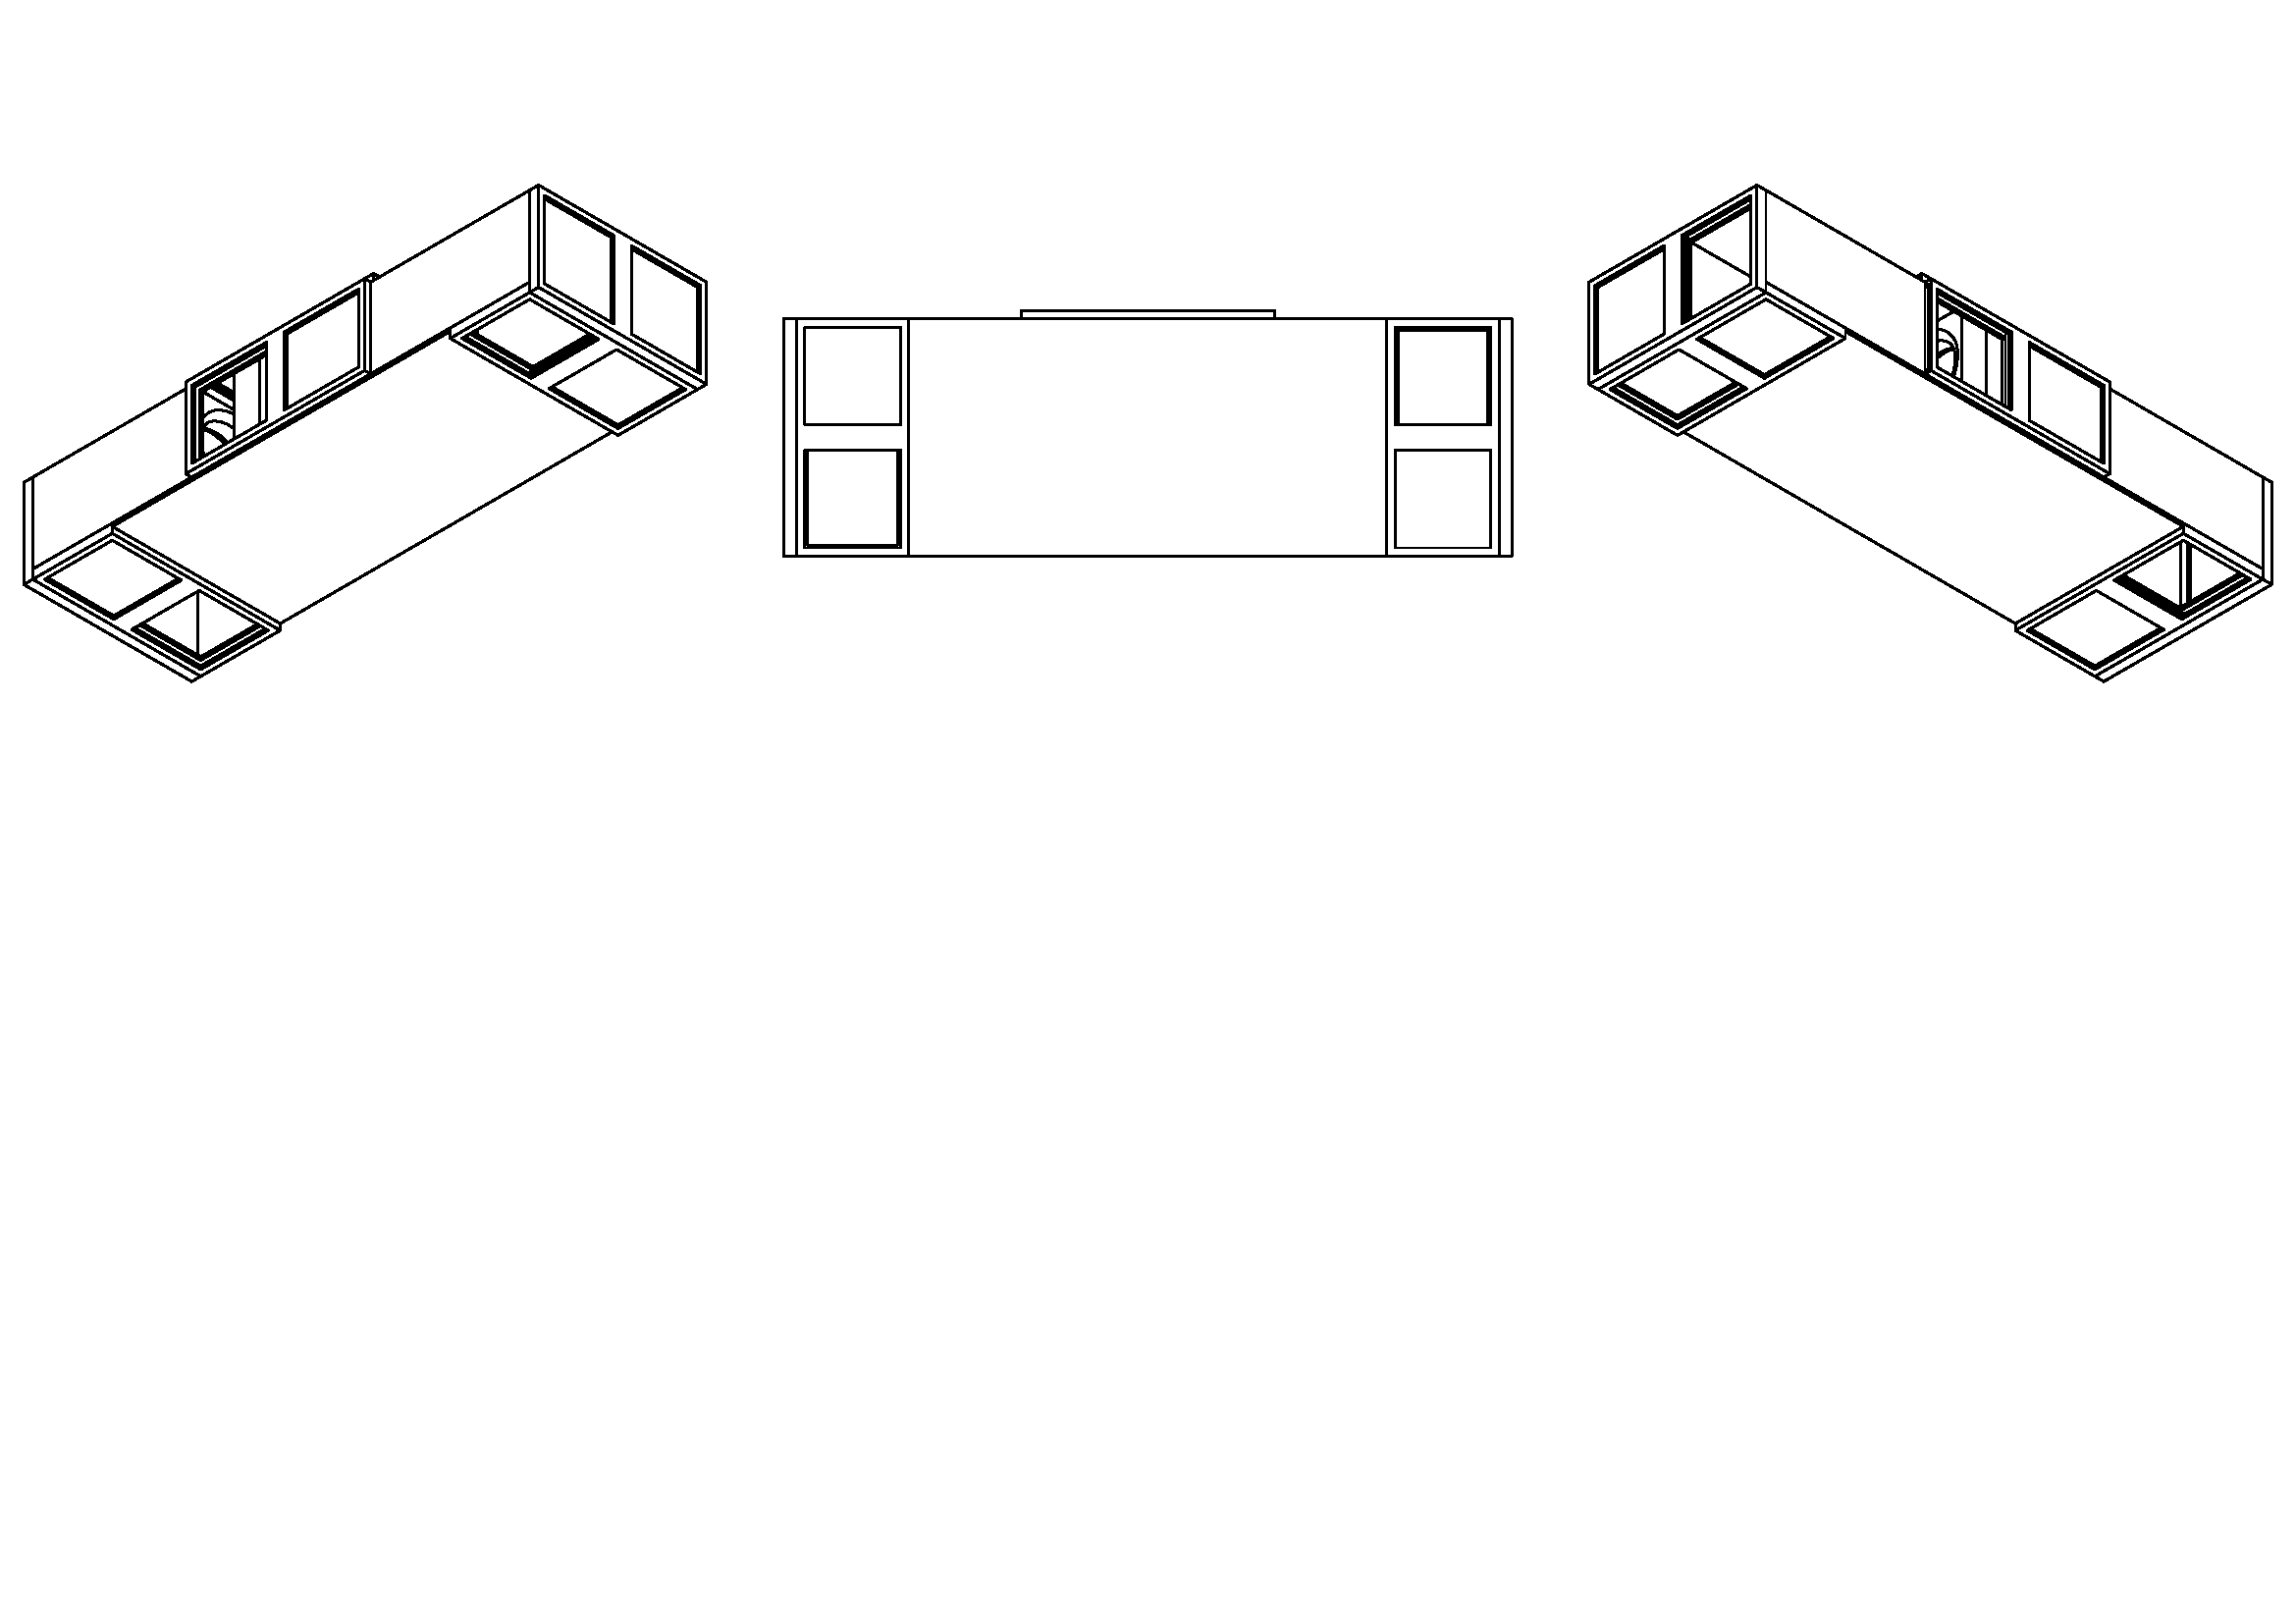
\includegraphics [
            trim = {0 16.0cm 0 3.15cm},
            clip,
        ] {\subfix{pics/cmode_bot.pdf}}
    }
    ;

    %% annotation bubbles

    \draw
    (#1-imgTop.north west) ++(2.5cm, -2.0cm) coordinate (#1-bOne)
    (#1-imgTop.north east) ++(-2.5cm, -2.0cm) coordinate (#1-bThree)

    (#1-imgTop.south west) ++(2.5cm, 2.0cm) coordinate (#1-bSeven)
    (#1-imgTop.south east) ++(-2.5cm, 2.0cm) coordinate (#1-bNine)

    (#1-imgBot.north west) ++(2.5cm, -1.5cm) coordinate (#1-bTen)
    (#1-imgBot.north east) ++(-2.5cm, -1.5cm) coordinate (#1-bTwelve)

    (#1-imgTop.west) ++(2.5cm, 0) coordinate (#1-bFour)
    (#1-imgTop.east) ++(-2.5cm, 0) coordinate (#1-bSix)

    (#1-imgTop.north) ++(0, -2.0cm) coordinate (#1-bTwo)
    ($(#1-imgTop.center)!0.5!(#1-imgTop.north)$) ++(0, -2.5cm) coordinate (#1-bFive)

    (#1-imgTop.south) ++(0, 2.0cm) coordinate (#1-bEight)

    (#1-imgBot.south) ++(0, 0.0cm) coordinate (#1-bEleven)
    ;


    \foreach \coord/\bubble in {
        #1-bEleven/11,
        #1-bEight/08,
        #1-bTwo/02,
        #1-bFive/05,
        #1-bFour/04,
        #1-bSix/06,
        #1-bTen/10,
        #1-bTwelve/12,
        #1-bSeven/07,
        #1-bNine/09,
        #1-bThree/03,
        #1-bOne/01%
    } {
        \draw [
            ultra thick,
        ]
        (\coord)
        node [
            font = \huge,
        ] {
            \texttt{\bubble}
        }
        (\coord) circle (\annoBubbleRadius)
        ;
    }



}

\subtikzpictureactivate{subCADExhaustCMODE}
